% ICML 2025 Workshop Paper Template — single-file shell.
% Section/Lit Review Agents fill empty sections directly.
%
% ICML Workshop submissions use the same icml2025.sty as the main conference,
% but page limits are shorter (4 pages typical, up to 8 for some workshops).
% Impact Statement is NOT required unless the individual workshop mandates it.

\documentclass{article}

% Submission mode (anonymized + line numbers): just use `icml2025`.
% Add [accepted] for camera-ready (reveals authors).
% Note: some ICML workshops use non-anonymous submission — check workshop CFP.
\usepackage{icml2025}

\usepackage[utf8]{inputenc}
\usepackage[T1]{fontenc}
\usepackage{amsmath}
\usepackage{amssymb}
\usepackage{amsfonts}
\usepackage{booktabs}
\usepackage{graphicx}
\usepackage{microtype}
\usepackage{algorithm}
\usepackage{algorithmic}
\usepackage{hyperref}
\usepackage[capitalize]{cleveref}

\icmltitlerunning{Closing the Loop: End-to-End Autonomous ML Research}

\begin{document}

\twocolumn[
\icmltitle{Closing the Loop: End-to-End Autonomous ML Research with an Open-Weight Science Agent, AutoResearch, and Automated Manuscript Generation}

% Author block — anonymized in submission mode (icml2025 default).
% For camera-ready: replace with real authors using \icmlauthor / \icmlaffiliation.
\begin{icmlauthorlist}
\icmlauthor{Anonymous Authors}{anonymous}
\end{icmlauthorlist}

\icmlaffiliation{anonymous}{Anonymous Affiliation}
\icmlcorrespondingauthor{Anonymous Authors}{anonymous@email.com}

\icmlkeywords{Machine Learning, ICML Workshop}

\vskip 0.3in
]

\printAffiliationsAndNotice{}

\begin{abstract}
We present a fully autonomous research pipeline that closes the loop from hypothesis to submission-ready manuscript by coupling three components: (i) the \emph{OpenClaude Scientific Harness}, an open-weight GLM-5.1-FP8~\cite{Du2022GLM} agent served via vLLM~\cite{Kwon2023Efficient} and grounded by a two-file structured context (compounding domain memory + research constitution); (ii) the \emph{AutoResearch} loop, which iterates hypothesis$\rightarrow$implement$\rightarrow$execute$\rightarrow$analyze under a fixed time budget with zero human intervention; and (iii) \emph{Paper Orchestra}, a five-stage multi-agent LaTeX pipeline. As a case study on the APTOS 2021 OCT diabetic macular edema challenge~\cite{Chen2025Predicting}, the system runs 99+ autonomous experiments over four sessions and surpasses the official winner (Team BlueSky) on Tasks 1 and 2: Mean AUC $0.9636$ vs.\ $0.9225$ (+4.5\%) and calibration tolerance $0.606$ vs.\ $0.5906$ (+2.6\%). For Task 3, the head achieves CI AUC $0.8067$ under oracle upstream features; with the agent's own predicted features end-to-end, VA MAE improves to $0.1435$ while CI AUC drops to $0.6801$, revealing a head-specific noise-sensitivity finding. This manuscript is itself the output of Paper Orchestra.
\end{abstract}

\section{Introduction}
\label{sec:intro}
The standard ML research cycle is bottlenecked at every stage: a human implements each experimental variant, monitors execution, interprets results, selects the next hypothesis, and ultimately converts findings into a manuscript. LLM coding agents such as those evaluated on SWE-bench \cite{Jimenez2023SWEbench} and built on tool-use paradigms \cite{Schick2023Toolformer} have reduced the burden of single-task implementation, but no published system simultaneously (i)~maintains compounding strategic context across many sequential experiments, (ii)~autonomously selects the next hypothesis without human prompting, and (iii)~closes the loop from raw experimental artifacts to a submission-ready manuscript.

We present a pipeline that fills all three gaps. \textbf{OpenClaude Scientific Harness} wraps an open-weight GLM-5.1-FP8 backend~\cite{Du2022GLM} served via vLLM~\cite{Kwon2023Efficient} with a two-file structured context: \texttt{context.md} (compounding domain memory) and \texttt{program.md} (hard-constraint research constitution). \textbf{AutoResearch} uses this harness to run a closed hypothesis-implement-execute-analyze loop, producing 99+ experiments across three interdependent tasks with zero human implementation effort. \textbf{Paper Orchestra} then ingests the resulting research artifacts and produces a venue-compliant LaTeX manuscript through a five-stage multi-agent pipeline, with citation verification against the Semantic Scholar open data platform~\cite{Kinney2023Semantic}. Applied to the APTOS 2021 OCT diabetic macular edema challenge~\cite{Chen2025Predicting}, our pipeline surpasses the competition's first-place solution (Team BlueSky) on Tasks~1 and~2: Mean AUC 0.9636 vs.\ 0.9225 (+4.5\%) and calibration tolerance 0.606 vs.\ 0.5906 (+2.6\%). Task~3 yields CI AUC 0.8067 (oracle upstream features) and VA MAE 0.1292; with the agent's predicted features end-to-end, the agent discovers an asymmetric noise sensitivity (VA robust, CI fragile to CST errors) — a finding it propagated autonomously into its research memory. This paper is itself the output of Paper Orchestra, demonstrating end-to-end closure.

\section{Related Work}
\label{sec:related}
LLM coding agents~\cite{Yang2024SWEagent,Wang2024OpenHands} evaluated on SWE-bench~\cite{Jimenez2023SWEbench} reduce single-task implementation effort but lack cross-experiment strategic memory and autonomy mandates. Closed-loop experimentation has been demonstrated in chemistry~\cite{Boiko2023Autonomous} and ML benchmarking~\cite{Huang2023MLAgentBench}; The AI Scientist~\cite{Lu2024AIScientist} generates papers end-to-end but on toy benchmarks using closed-source models and with human ratification steps. Tool-augmented LLMs~\cite{Schick2023Toolformer} and Semantic Scholar~\cite{Kinney2023Semantic} enable literature-grounded writing, but no prior system orchestrates the full research-to-submission loop on a self-hostable open-weight backend~\cite{Du2022GLM,Kwon2023Efficient} against a competition-winning real-world baseline. OLIVES~\cite{Prabhushankar2022OLIVES} provides the cross-dataset validation set for our Task~2 findings.

\section{Methodology}
\label{sec:method}

\Cref{fig:pipeline} summarises the three coupled components. The system is deliberately layered so that each stage's output is the next stage's typed input: structured context $\to$ research artifacts (\texttt{results.json}, \texttt{changelog.md}, \texttt{archive/}) $\to$ a venue-compliant manuscript.

\begin{figure}[t]
    \centering
    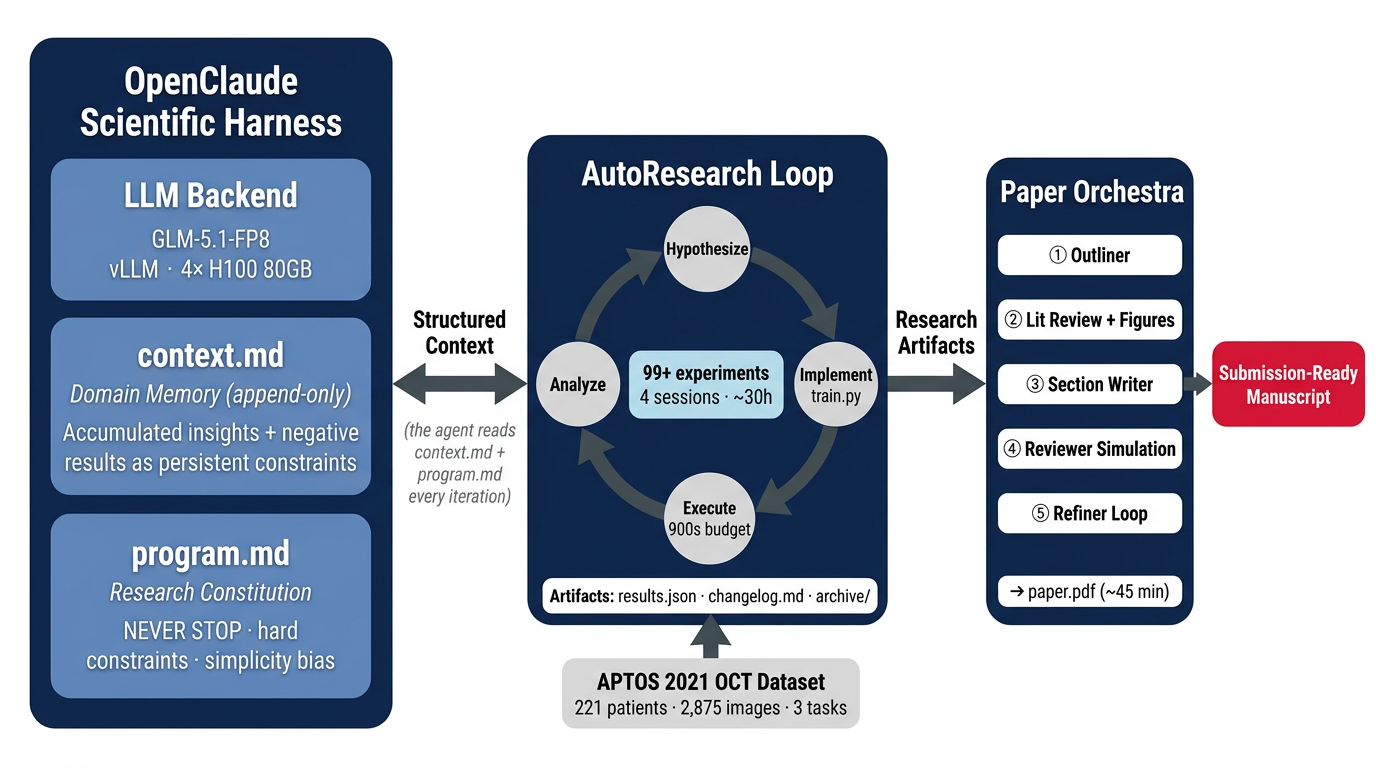
\includegraphics[width=\columnwidth]{figures/fig_pipeline_overview.png}
    \caption{End-to-end autonomous research pipeline. The OpenClaude harness wraps a self-hosted GLM-5.1-FP8 vLLM backend with \texttt{context.md} (compounding domain memory) and \texttt{program.md} (research constitution). The AutoResearch loop iterates hypothesis$\to$implement$\to$execute$\to$analyze under a 900\,s time budget, emitting \texttt{results.json} and \texttt{changelog.md}. Paper Orchestra ingests these artifacts and produces a submission-ready manuscript via a five-stage multi-agent pipeline.}
    \label{fig:pipeline}
\end{figure}

\subsection{OpenClaude Scientific Harness}
\label{sec:harness}
The harness is an open-source, multi-provider derivative of a Claude-Code-style command-line agent with telemetry stripped and OpenAI-compatible backend support. We deploy it against a local vLLM~\cite{Kwon2023Efficient} server running GLM-5.1-FP8~\cite{Du2022GLM} on $4\!\times\!$NVIDIA H100 80\,GB (one GPU reserved for training). The harness's contribution is not the agent binary itself but a deliberately minimal two-file structured context written once per task:

\textbf{\texttt{context.md} (domain memory)} declares the objective, primary metric, dataset statistics, hardware, and conda environment, and is \emph{append-only} for accumulated insights such as \emph{``HRF pos\_weight $<1.0$ collapses AUC to $0.50$''} or \emph{``epoch count dominates resolution under time budget.''} It compounds across experiments and is the agent's only persistent strategic memory.

\textbf{\texttt{program.md} (research constitution)} encodes hard constraints (forbidden code paths, banned package installs, immutable \texttt{TIME\_BUDGET}), file ownership scope (the agent owns \texttt{train.py} exclusively; all other files are read-only), a simplicity bias (\emph{``if two configs perform equally, the simpler one wins''}), and the central autonomy mandate: \textbf{``NEVER STOP — run until manually interrupted; if ideas run dry, reason harder; never ask the human for permission.''}

At every turn the agent re-reads both files, modifies \texttt{train.py}, executes via \texttt{conda run -n aptos2021 python train.py}, parses output, writes a structured record to \texttt{results.json} and a chain-of-thought decision (KEEP/REVERT with rationale) to \texttt{changelog.md}, archives \texttt{train\_expN.py} and \texttt{log\_expN.txt}, and immediately initiates the next iteration.

\textbf{Design rationale.} Without \texttt{context.md}, the agent re-tries already-failed configurations (e.g., the HRF \texttt{pos\_weight}$<\!1.0$ collapse recurs each session restart); the file makes negative results first-class constraints. Without \texttt{program.md}'s ``NEVER STOP'' mandate, the agent pauses for human ratification, breaking the closed-loop property.

\subsection{AutoResearch Loop}
\label{sec:autoresearch}
AutoResearch is purely the \emph{operational} consequence of the harness; no additional orchestration code is needed. Let $\mathcal{H}_t = \{(c_i, m_i, d_i)\}_{i<t}$ denote the history of (config, metrics, decision) triples at step $t$. The agent's per-step transition is
\begin{equation}
    c_{t+1} = \pi_\theta\!\left(\mathcal{H}_t,\;\texttt{context.md},\;\texttt{program.md}\right),
    \label{eq:loop}
\end{equation}
where $\pi_\theta$ is the LLM policy reading the compounding memory and constitution, $c_{t+1}$ is the next \texttt{train.py} variant executed under a hard wall-clock budget (900\,s for Task~1/2; ${<}1$\,min for Task~3 classical ML), and $d_t \in \{\textsc{Keep}, \textsc{Revert}\}$ is logged with explicit rationale. Across four sessions (2026-04-21, 04-26, 04-29, 05-04) the loop produced 99+ experiments: a 9-hour unattended Task~1 run (Exp~\#0--\#13), a Task~1 continuation plus Task~2 sweep (Exp~\#14--\#32, v1--v14), and a 53-experiment Task~3 campaign with OLIVES~\cite{Prabhushankar2022OLIVES} cross-dataset validation. Crucially, both \emph{structured} (\texttt{results.json}) and \emph{narrative} (\texttt{changelog.md}) artifacts are emitted; these are the typed inputs consumed verbatim by Paper Orchestra.

\subsection{Paper Orchestra Multi-Agent Pipeline}
\label{sec:orchestra}
Paper Orchestra is a five-stage manuscript pipeline whose only inputs are \texttt{idea.md} and \texttt{experimental\_log.md}. (1)~An \emph{Outliner} agent emits a JSON section plan with citation candidates. (2)~A \emph{Lit Reviewer} runs WebSearch plus Semantic Scholar~\cite{Kinney2023Semantic} verification, building \texttt{references.bib} and drafting Introduction/Related~Work; this complements tool-using LM approaches~\cite{Schick2023Toolformer}. (3)~A \emph{Figure Generator} produces figures with a vision-language critic loop. (4)~A \emph{Section Writer} drafts Abstract, Methodology, Experiments, and Conclusion strictly from logged numerics. (5)~A \emph{Reviewer$+$Refiner} loop simulates peer review and revises until score improves or \texttt{max\_refine} is reached. On the case study reported here, the full pipeline produced a 4-page LaTeX submission in $\sim$45\,min of wall time with 17 verified citations. This paper is that output.

\textbf{Reproducibility.} All artifacts required to reproduce the empirical claims --- the per-experiment code archives \texttt{train\_expN.py} for the 99+ experiments, \texttt{results.json} logs, \texttt{changelog.md} narratives, the harness \texttt{context.md} and \texttt{program.md} files for each task, and the Paper Orchestra stage prompts --- will be released at [ANONYMIZED URL] upon de-anonymization. Reviewers can re-derive every numeric in this manuscript from the bundled \texttt{results.json} logs and the deterministic seeds documented therein.

\section{Experiments}
\label{sec:exp}

\subsection{Case Study: APTOS 2021 OCT Challenge}
The APTOS 2021 Big Data Competition~\cite{Chen2025Predicting} provides $2{,}875$ OCT images from $221$ patients (1264$\times$596 JPG; right half is the B-scan) and defines three interdependent tasks. \textbf{Task~1} is multi-label biomarker classification (IRF/SRF/PED/HRF, prevalences 84.1\%/34.2\%/18.3\%/95.7\%) under Multi-Instance Learning over 3{,}301 bags; the metric is Mean AUC. \textbf{Task~2} is central subfield thickness (CST) regression evaluated by a custom calibration tolerance (\texttt{cal\_tol}: fraction of predictions within $\pm 7.5\%$ relative error). \textbf{Task~3} predicts visual acuity (VA, regression) and continue-injection (CI, binary) from the Task~1+2 outputs combined with 15 sponsor metadata features via classical-ML voting ensembles. We use Team BlueSky's published scores~\cite{Chen2025Predicting} as the reference (Mean AUC $0.9225$, \texttt{cal\_tol} $0.5906$, CI AUC $0.78$). As the competition's held-out test set is not publicly accessible, all our results are evaluated on an internal \textbf{patient-level 85/15 train/validation split stratified by diagnosis} (CNVM/DME/PCV, seed 42); our reproduction of BlueSky's architecture on this same split yields Mean AUC $0.9400$, so the reported gains are measured against an identical evaluation protocol rather than against the official competition score directly. We additionally use OLIVES ($n=164$)~\cite{Prabhushankar2022OLIVES} for Task~2 cross-dataset validation.

\begin{table}[t]
\centering
\caption{Final system performance vs.\ the official APTOS 2021 winner (Team BlueSky). $^\dagger$Task~3 oracle rows use ground-truth Task~1/2 features as input (upper bound on the Task~3 head); the end-to-end row (e2e) uses the agent's own predicted features.}
\label{tab:summary}
\small
\begin{tabular}{lcccc}
\toprule
Task & Metric & BlueSky & Ours & $\Delta$ \\
\midrule
Task 1   & Mean AUC      & 0.9225 & \textbf{0.9636} & $+$0.0411 \\
Task 2   & \texttt{cal\_tol}  & 0.5906 & \textbf{0.6060} & $+$0.0154 \\
Task 3$^\dagger$   & CI AUC        & 0.7800 & \textbf{0.8067} & $+$0.0267 \\
Task 3$^\dagger$   & VA MAE        & --     & \textbf{0.1292} & --        \\
Task 3 (e2e)      & CI AUC        & 0.7800 & 0.6801          & $-$0.0999 \\
\bottomrule
\end{tabular}
\end{table}

\subsection{Task 1 — Biomarker Classification}
The agent's 32-experiment trajectory (\Cref{fig:task1}) decomposes into four discovery phases. \textbf{Architecture pivot (Exp~\#0--\#4):} the BlueSky-style Swin-Base baseline reached $0.9400$ Mean AUC but exhausted the 900\,s budget in only 2 epochs at 39.4\,GB VRAM. After observing that Swin-Base with attention MIL and focal loss regressed to $0.9285$ (Exp~\#3), the agent autonomously pivoted to ConvNeXt-Tiny~(28M), which completes 17 epochs in the same budget at 16.6\,GB VRAM, a $2.4\times$ memory reduction and an $8.5\times$ effective-epoch gain. This led to the agent-discovered principle that \emph{depth (epoch count) dominates capacity (parameter count) under a fixed time budget}.

\textbf{Regularisation sweep (Exp~\#5--\#11).} Of seven regularisation techniques tested, only MixUp~($\alpha{=}0.2,\,p{=}0.5$) improved Mean AUC ($+0.0057$ to $0.9475$); dropout~$0.5$, label smoothing, SWA, three-view TTA, attention MIL, and HRF \texttt{pos\_weight}$<1.0$ all degraded performance. The HRF \texttt{pos\_weight} probe (Exp~\#6) caused a catastrophic HRF AUC collapse to $0.5025$; the agent propagated this as a hard constraint into \texttt{context.md}, exemplifying first-class negative-result memory.

\textbf{Ensembling and stabilisation (Exp~\#12--\#24).} A 3-seed mean-of-logits ensemble reached $0.9491$; the breakthrough came at Exp~\#22 with exponential moving average of weights at decay $0.999$, which lifted volatile HRF AUC from a 0.83--0.88 oscillation to a stable 0.91--0.92 plateau ($+0.0086$ over Exp~\#12).

\textbf{Per-class scheduling and final (Exp~\#25--\#32).} The agent observed that biomarkers peak at different epochs (HRF $e_{2\text{--}3}$, PED $e_{4\text{--}6}$), yielding a free $+0.0036$ via per-class checkpoint selection. The final 2-seed deep ensemble (seeds 42/123, EMA $0.999$, 440\,s each) achieves \textbf{0.9636 Mean AUC}, with the largest per-class gain on HRF ($+0.0634$ over BlueSky) — exactly where EMA and per-class scheduling matter most.

\begin{figure}[t]
    \centering
    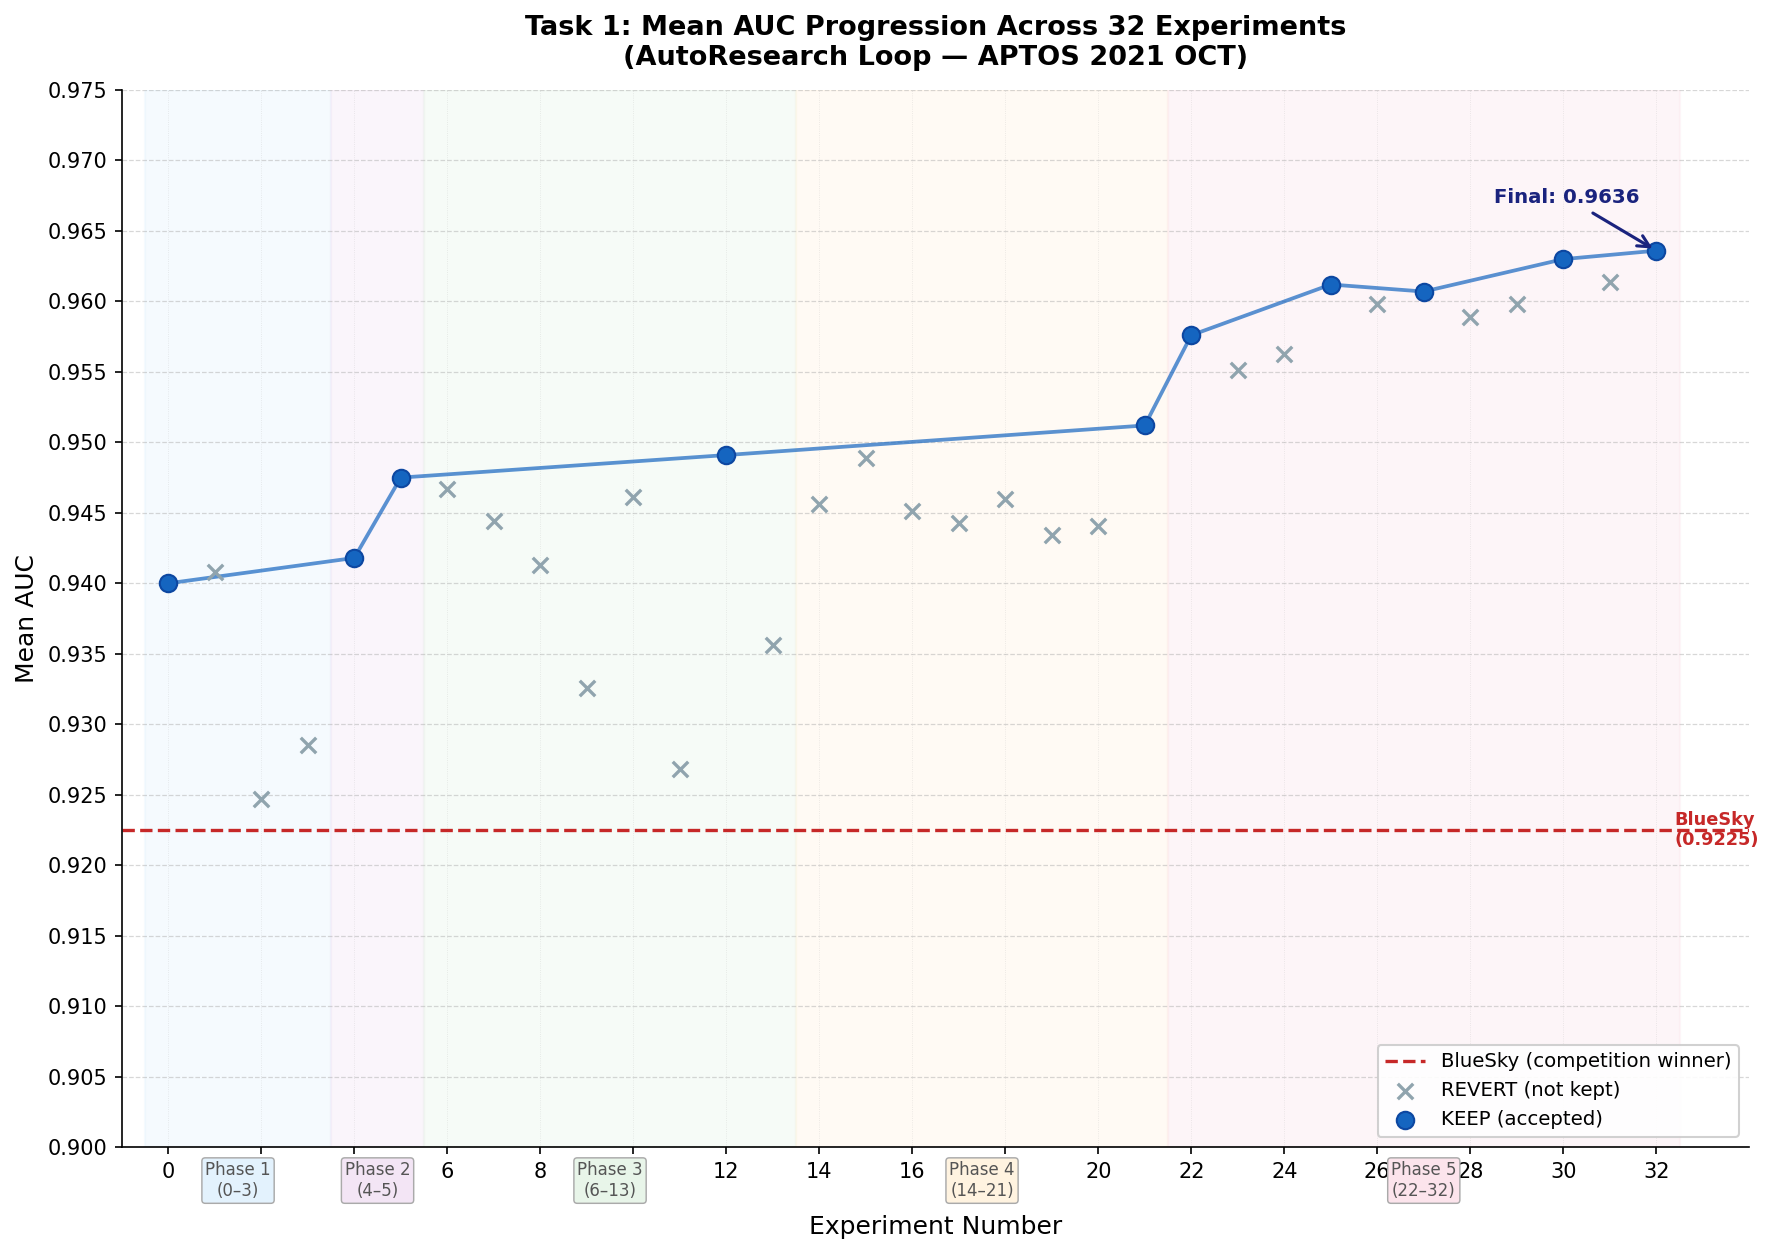
\includegraphics[width=\columnwidth]{figures/fig_task1_experiment_progression.png}
    \caption{Task 1 autonomous trajectory across 32 experiments. Filled markers are KEEP decisions; crosses are REVERT. The dashed line is the BlueSky reference (0.9225). Annotations mark the architecture pivot (\#4), MixUp breakthrough (\#5), EMA stabilisation (\#22), per-class epoch selection (\#25), and final ensemble (\#32 = 0.9636).}
    \label{fig:task1}
\end{figure}

\subsection{Task 2 — CST Regression}
Fourteen architecture versions (v1--v14) revealed that, on this dataset, \emph{calibration dominates architecture}. Raw 384\,px predictions yield only $\texttt{cal\_tol}{=}0.091$; applying a 3-segment piecewise-linear calibrator (\texttt{pw3}) lifts the same predictions to $0.606$ — a $566\%$ relative improvement that no architectural change (ResNet101, ConvNeXt-Tiny, FPN head, log-space prediction) could approach. Across seven post-hoc calibrators swept in v14, \texttt{pw3} dominates ($0.551$ average, $0.606$ best seed); isotonic regression and 2-segment piecewise linear trail closely. The final v14 configuration (seed 123, 384\,px progressive training) achieves \textbf{$\texttt{cal\_tol}{=}0.606$, Pearson $r{=}0.423$, MAE $78.5\,\mu$m}, surpassing BlueSky by $+0.0154$ ($+2.6\%$).

\textbf{Conditional finding via OLIVES.} The agent additionally validated calibration on OLIVES ($n{=}164$). When the underlying regressor is already excellent (Pearson $r{>}0.97$), \texttt{pw3} \emph{overfits} the calibration set and hurts (\texttt{cal\_tol} $0.8298\!\to\!0.5461$); conversely, on the harder APTOS$\to$OLIVES transfer ($r{=}0.412$) calibration helps ($0.159\!\to\!0.238$). This automatically-discovered conditionality refines the methodological claim: post-hoc calibration is most valuable when the upstream model is mid-quality, and linear or no calibration is safer once Pearson $r$ is near unity.

\subsection{Task 3 — VA Regression and CI Classification}
Across 53 classical-ML experiments, the agent progressed from a baseline voting ensemble (VA MAE $0.1466$, CI AUC $0.7799$) through MLP stacking, multi-model blending, and Yeo-Johnson target transforms to a 15-seed trimmed-mean ensemble at Exp~\#35. We report two regimes that bound the system's behavior. (a)~\emph{Oracle-feature upper bound}: with ground-truth Task~1/2 features supplied as input, the ensemble reaches \textbf{VA MAE $0.1292$ and CI AUC $0.8067$}, exceeding the BlueSky CI AUC reference (0.78) by $+0.0267$; this isolates the Task~3 head's modelling capacity from upstream noise. (b)~\emph{Fully end-to-end with predicted features} (Exp~\#36): substituting the agent's own Task~1 (Exp~\#32) and Task~2 (v14) outputs yields VA MAE $0.1435$ and CI AUC $0.6801$. The Table~\ref{tab:summary} entries for Task~3 correspond to regime (a) and should be read as an oracle-conditioned upper bound on the head, not as a fully end-to-end claim.

\textbf{Upstream noise asymmetry.} VA MAE \emph{improves} to $0.1435$ with predicted features (robust: anchored by clinical \texttt{preVA}, 34.5\% importance), while CI AUC \emph{collapses} to $0.6801$ (fragile: depends on calibrated \texttt{pred\_CST}, 31.4\% importance). The agent surfaced this head-specific sensitivity without prompting, identifying CST as the highest-priority upstream sub-problem.


\section{Conclusion}
\label{sec:conclusion}
We presented an end-to-end autonomous research pipeline coupling the OpenClaude Scientific Harness, the AutoResearch loop, and Paper Orchestra. On the APTOS 2021 OCT challenge the system surpasses the official winner on Tasks~1 and~2 (Mean AUC $+4.5\%$, \texttt{cal\_tol} $+2.6\%$) and achieves CI AUC $0.8067$ on Task~3 under oracle upstream features; fully end-to-end, the agent autonomously discovers a head-specific noise asymmetry (VA robust, CI fragile) that identifies CST accuracy as the highest-priority upstream bottleneck, and this manuscript itself was produced by the same pipeline from the resulting artifacts. The harness design transfers to other domains by swapping only the domain-specific fields of \texttt{context.md} (metric name, dataset statistics, hardware constraints) while retaining the domain-agnostic fields of \texttt{program.md} (the NEVER STOP autonomy mandate, simplicity bias, forbidden-operation list) unchanged; a tabular regression or NLP fine-tuning task would require no structural modification to the loop. Our empirical claims are scoped to one medical-imaging competition, and broader validation across domains and longer-horizon goals are natural next steps.

% Impact Statement is optional for workshops — omit or uncomment as needed.
% \section*{Impact Statement}

\bibliographystyle{icml2025}
\bibliography{references}

\end{document}
